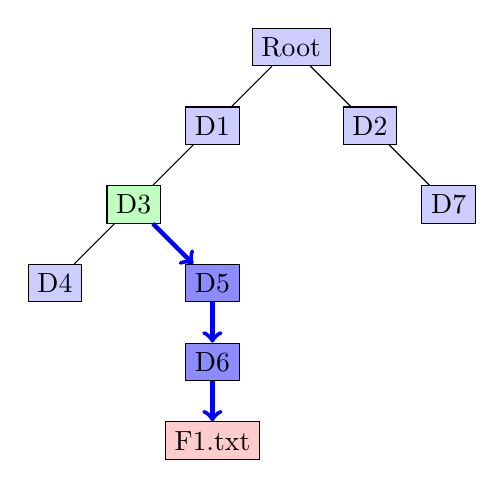
\begin{tikzpicture}[directory/.style={rectangle,draw,fill=blue!20},
				file/.style = {rectangle, draw, fill=red!20},
				directoryC/.style={rectangle, draw, fill=green!25},
				directoryR/.style={rectangle, draw, fill=blue!45}]
	\node[directory] (R) at  (0,0) {Root};
	\node[directory] (D1) at (-1,-1) {D1};
	\node[directory] (D2) at (1,-1) {D2};
	\node[directoryC] (D3) at (-2,-2) {D3};
	\node[directory] (D7) at (2,-2) {D7};
	\node[directory] (D4) at (-3,-3) {D4};
	\node[directoryR] (D5) at (-1,-3) {D5};
	\node[directoryR] (D6) at (-1,-4) {D6};
	\node[file] (F1) at (-1,-5) {F1.txt};
	\draw[-] (R) -- (D1);
	\draw[-] (R) -- (D2);
	\draw[-] (D1) -- (D3);
	\draw[-,] (D3) -- (D4);
	\draw[->, color = blue, ultra thick] (D3) -- (D5);
	\draw[->, color = blue, ultra thick] (D5) -- (D6);
	\draw[->, color = blue, ultra thick] (D6) -- (F1);
	\draw[-] (D2) -- (D7);
\end{tikzpicture}

